\chapter{Intégration}
\labch{integration}

\section{Fonction intégrable et décroissante sur \texorpdfstring{$\R^+$}{R+}}
\begin{exercice}
    \marginnote[0cm]{Source : \cite{exos_oraux} p. 268}
    Soit $f : \Rp \to \R$ une fonction continue, décroissante et intégrable. Montrer que $x f(x) \xrightarrow[x \to +\infty]{} 0$.
\end{exercice}

\todoinline{On pourrait faire un dessin pour les  points 1 et 2 qui sont classique mais pas très bien compris en minorant/majorant l'aire sous $f$ par l'aire d'un rectangle. On peut aussi illustrer l'encadrement final.}


\begin{elem_sol}
\begin{itemize}
\item Comme $f$ est décroissante, d'après le théorème de la limite monotone, il existe $\ell \in \R \cup \ens{-\infty}$ tel que $\lim\limits_{x\to+\infty} f(x) = \ell$.

\item Montrons par l'absurde que $f$ est positive. S'il existe $x_0 \geq 0$ tel que $f(x_0) < 0$, comme $f$ est décroissante,
\[
\forall\ x \geq x_0,\, f(x) \leq f(x_0).
\]
Ainsi,
\[
\forall\ x \geq x_0,\, \displaystyle\int_{x_0}^x f(t) \mathrm{d}t \leq f(x_0) (x - x_0).
\]
D'après le théorème d'encadrement, $\lim\limits_{x\to+\infty} \displaystyle\int_{x_0}^x f(t) \mathrm{d}t = -\infty$, ce qui est impossible car $f$ est intégrable. Ainsi, $f$ est à valeurs positives et $\ell \geq 0$.

\item Supposons par l'absurde que $\ell > 0$. Alors, il existe un réel $A$ tel que
\[
\forall\ x \geq A,\, f(x) \geq \frac{\ell}{2}.
\]
Ainsi,
\[
\forall\ x \geq A,\, \displaystyle\int_A^x f(t) \mathrm{d}t \geq \frac{\ell}{2} (x - A).
\]
D'après le théorème d'encadrement, $\lim\limits_{x\to+\infty} \displaystyle\int_A^x f(t) \mathrm{d}t = +\infty$, ce qui est impossible car $f$ est intégrable.

Finalement, $\lim\limits_{x\to+\infty} f(x) = 0$.

\item Soit $x \geq 0$. Comme $f$ est décroissante,
\[
\displaystyle\int_x^{2 x} f(t) \mathrm{d}t \leq (2 x - x) f(x).
\]

De même,
\[
\displaystyle\int_{x/2}^x f(t) \mathrm{d}t \geq \frac{x}{2} f(x).
\]

Ainsi,
\[
\displaystyle\int_x^{2 x} f(t) \mathrm{d}t \leq x f(x) \leq 2 \displaystyle\int_{x/2}^x f(t) \mathrm{d}t.
\]
En notant $F : x \mapsto \displaystyle\int_0^x f(t) \mathrm{d}t$, comme $F$ est intégrable, alors $F$ possède une limite finie en $+\infty$.

Alors,
\[
F(2 x) - F(x) \leq x f(x) \leq 2 (F(x) - F(x/2)).
\]

Ainsi, d'après le théorème d'encadrement, $\lim\limits_{x\to 0} x f(x) = 0$.
\end{itemize}

\begin{itemize}
\item Montrer que $f$ tend vers 0 en utilisant sa décroissance et son intégrabilité. $f$ est donc à valeurs positives. 
\item Encadrer $x f(x)$ en écrivant $x=2 \cdot \frac{x}{2}$.
\end{itemize}
\end{elem_sol}

\todoinline{Ajouter une illustration avec une fonction type Riemann ?}

\begin{exercice}
    \marginnote[0cm]{Source : \cite{truc2019} p. 268}
    Soit $f : ]0, 1] \to \R$ une fonction continue, décroissante et intégrable. Alors,
    \[
    \lim\limits \frac{1}{n} \sum\limits_{k=1}^n f\left(\frac{k}{n}\right) = \displaystyle\int_0^1 f(t) \mathrm{d}t.
    \]
\end{exercice}

\begin{elem_sol}
On note $R_n(f) = \frac{1}{n} \sum\limits_{k=1}^n f\left(\frac{k}{n}\right)$.
\begin{itemize}
\item Soit $n \geq 1$. On utilise la décroissance de la fonction $f$, pour tout $k \leq t \leq k + 1 \leq n-1$,
\begin{align*}
\frac{1}{n} f\left(\frac{k+1}{n}\right) &\leq \displaystyle\int_{k/n}^{(k+1)/n} f(t) \mathrm{d}t \leq \frac{1}{n} f\left(\frac{k}{n}\right)\\
\frac{1}{n} \sum\limits_{k=2}^{n} f\left(\frac{k}{n}\right) &\leq \displaystyle\int_{1/n}^1 f(t) \mathrm{d}t \leq \frac{1}{n} \sum\limits_{k=1}^{n-1} f\left(\frac{k}{n}\right)\\
R_n - \frac{1}{n} f\left(\frac{1}{n}\right) &\leq \displaystyle\int_{1/n}^1 f(t) \mathrm{d}t \leq R_n - \frac{f(1)}{n}.
\end{align*}

Ainsi,
\begin{align*}
\displaystyle\int_{1/n}^1 f(t) \mathrm{d}t + \frac{f(1)}{n} &\leq R_n \leq \displaystyle\int_{1/n} f(t) \mathrm{d}t + \frac{1}{n}  f\left(\frac{1}{n}\right).
\end{align*}

\item Comme $f$ est décroissante et intégrable sur $]0, 1]$,
\[
\frac{1}{n} f\left(\frac{1}{n}\right) \leq \displaystyle\int_0^{1/n} f(t) \mathrm{d}t.
\]

\item Comme $f$ est intégrable sur $]0, 1]$,
\[
\lim\limits_{n\to+\infty} \displaystyle\int_{1/n}^1 f(t) \mathrm{d}t = \displaystyle\int_0^1 f(t) \mathrm{d}t.
\]
\end{itemize}

Ainsi, d'après le théorème d'encadrement,
\[
\lim\limits_{n\to+\infty} R_n(f) = \displaystyle\int_0^1 f(t) \mathrm{d}t.
\]
\end{elem_sol}


\todoinline{On peut éventuellement ajouter l'exercice suivant. Il s'agit d'une somme de Riemann mais sur $[1, +\infty[$}
%---------------

\begin{exercice}
\cite{RMS 888 2016 - ENSAM}
Soit $f : x \mapsto \frac{1}{x \sqrt{x^2 - 1}}$ définie sur $]1, +\infty[$.
\begin{enumerate}
\item Étudier et tracer la fonction $f$.

\smallskip
Pour tout entier naturel $n$, on pose $S_n = \sum\limits_{k=n+1}^{+\infty} \frac{1}{k \sqrt{k^2 - n^2}}$.
\item Étudier la convergence et la limite de la suite $(S_n)$.

\item Même question avec la suite $(n S_n)$.
\end{enumerate}
\end{exercice}

\begin{elem_sol}
\begin{enumerate}
\item $f$ est décroisante, à valeurs positives, $\lim\limits_{1^+} f = +\infty$ et $\lim\limits_{+\infty} f = 0$. De plus, $f$ est continue et dérivable.

\item D'après la définition de $f$,
\[
S_n = \frac{1}{n^2} \sum\limits_{k=n+1}^{+\infty} f(k/n).
\]
Comme $f$ est décroissante, pour tout $t \in [k/n,(k+1)/n]$,
\begin{align*}
f((k+1)/n) &\leq f(t) \leq f(k/n) \\
n^{-1} \sum\limits_{k=n+2}^{N+1} f(k/n) &\leq \displaystyle\int_{1+1/n}^{N/n} f(t) \mathrm{d}t \leq n^{-1} \sum\limits_{k=n+1}^{N} f(k/n).
\end{align*}
Comme $f(x) \sim_{+\infty} \frac{1}{x^2}$, la suite $(S_{n,N})_N$ est croissante et majorée par $\displaystyle\int_{1+1/n}^{+\infty} f(t) \mathrm{d}t$ qui est convergente. Ainsi, en passant à la limite dans l'inégalité,
\begin{align*}
n S_n - f((n+1)/n) &\leq \displaystyle\int_{1+1/n}^{+\infty} f(t) \mathrm{d}t \leq n S_n \\
\frac{1}{n} \displaystyle\int_{1+1/n}^{+\infty} f(t) \mathrm{d}t &\leq S_n \leq \frac{1}{n} \displaystyle\int_{1+1/n}^{+\infty} f(t) \mathrm{d}t + \frac{1}{n^2} f((n+1)/n).
\end{align*}
De plus, $f(x) \sim_1 \frac{1}{\sqrt{2 (x - 1)}}$, donc $f$ est intégrable en $1$ et $(S_n)$ converge vers $0$ car $f((n+1)/n) \sim n^{1/2}$.

\item En reprenant l'encadrement précédent, $\left(n^{-1} f((n+1)/n)\right)$ converge toujours vers $0$ et $(n S_n)$ converge vers $\displaystyle\int_1^{+\infty} f(t) \mathrm{d}t$.

\textbf{Remarque.} $\displaystyle\int^x f(t) \mathrm{d}t = - \arctan\frac{1}{\sqrt{x^2 - 1}}$ et $\displaystyle\int_1^{+\infty} f = \frac{\pi}{2}$.
\end{enumerate}
\end{elem_sol}

\section{Calcul d'une intégrale impropre}
\todoinline{Semble s'appeler l'intégrale d'Euler - \url{https://fr.wikipedia.org/wiki/Table_d'intégrales}}

\begin{exercice}
\cite{Oraux - CCP-PSI-2016}
\begin{enumerate}
\item Montrer que $I$ et $J$ sont convergentes et que $I = J$.
\item Calculer $I + J$ et en déduire $I$ et $J$.
\end{enumerate}
    % Calculer $\displaystyle \int_0^\pi \ln(\sin t) \d t.$
\end{exercice}

\todoinline{Ajouter une représentation graphique de la fonction ?}

\begin{elem_sol}
Soient $I = \int_0^{\pi/2} \ln(\sin(t)) \mathrm{d} t$ et $J = \int_0^{\pi/2} \ln(\cos(t)) \mathrm{d} t$.

\begin{enumerate}
\item La fonction $t \mapsto \ln(\sin(t))$ est continue sur $]0,\pi/2]$. De plus,
\[
\ln(\sin(t)) = \ln(t + o(t)) = \ln(t) + \ln(1 + o(1)) = o(\ln(t)).
\]
Ainsi, $t \mapsto \ln(\sin(t))$ est intégrable en $0$.

La formule de changement de variable, avec $\phi : u \mapsto \pi/2 - u$ assure la convergence de $J$ ainsi que l'égalité $I = J$.

\item Comme ces intégrales sont bien définies, en utilisant la relation de Chasles et la symétrie dans la dernière égalité,
\[
I + J = \int_0^{\pi/2} \ln\left(\frac{\sin(2t)}{2}\right) \mathrm{d} t = \frac{1}{2} \int_0^\pi \ln(\sin(t)) \mathrm{d} t - \frac{\pi}{2} \ln(2) = I - \frac{\pi}{2} \ln(2).
\]
Ainsi, $I = J = -\frac{\pi}{2} \ln(2)$.
\end{enumerate}
\end{elem_sol}

    

\section{Intégrales de  \textsc{Bertrand}}
\begin{prop}
    Soient $(\alpha, \beta) \in  \R^2$ et $f:t \to \frac{1}{t^{\alpha} \ln^{\beta} (t)}$. Alors,
    $$\int_{2}^{+ \infty} f \text{ converge si et seulement si }
    \begin{cases}
    \alpha > 1 \\
    \text{ou}\\
    \alpha = 1 \text{ et } \beta > 1
    \end{cases}.
    $$
\end{prop}

\textcolor{red}{à rerédiger}
\begin{preuve}
    Distinguons trois cas selon les valeurs prises par $\alpha$:
    \begin{enumerate}
        \item si $\alpha > 1$, soit $\gamma \in ]1, \alpha[$. On peut montrer que $$\displaystyle \frac{1}{t^{\alpha} \ln^{\beta} (t)} = o_{+ \infty} \left( \frac{1}{t^{\gamma}} \right).$$
        \item si $\alpha < 1$, soit $\gamma \in ]\alpha, 1[$. On peut montrer que 
        $ t^{\gamma} f(t) \xrightarrow[t \to + \infty]{} + \infty $
        donc à partir d'un certain rang, $f(t) \geqslant \frac{1}{t^{\gamma}} > 0$.
        \item si $\alpha = 1$, revenir aux intégrales partielles. Connaître la primitive de $t \mapsto \frac{1}{t \ln^{\beta} (t)}$:
        $$\int_{2}^{X} \frac{1}{t \ln^{\beta} (t)} \d t = 
        \begin{cases}
            \left[ \frac{\ln ^{1-\beta} (t)}{1-\beta} \right]_2 ^X & \text{si } \beta \not = 1, \\
            \left[\ln (\ln(t)) \right]_2 ^X & \text{si } \beta = 1.
        \end{cases}
        $$
        On en déduit que l'intégrale de la fonction $t \mapsto \frac{1}{t \ln^{\beta} (t)}$ converge sur $[2, + \infty[$ si et seulement si $\beta > 1$.
    \end{enumerate}
\end{preuve}


\section{Une propriété géométique de l'intégrale}
Soit $f$ de classe $\mathscr{C}^1$ sur $[a, b]$ telle que $f'$ soit strictement positive sur $[a, b]$. Calculer:
$$\int_{a}^{b} f(t)\ \d t + \int_{f(a)}^{f(b)} f^{-1}(t)\ \d t.$$

\begin{itemize}
    \item Justifier que $f^{-1}$ est licite. 
    \item Calculer le deuxième terme en posant $t = f(u)$.
    \item Effectuer une IPP sur le deuxième terme pour conclure. 
    Donner une interprétation géométrique.
\end{itemize}

\section{Permutation somme/intégrale}
Justifier les convergences, puis l'égalité:
$$\sum_{n=0}^{+ \infty} \frac{(-1)^n (2n+1)}{(2n+1)^2 + x^2} = \frac{1}{2} \int_{0}^{+ \infty} \frac{\cos (xt)}{\ch t}\ \d t.$$

\begin{itemize}
    \item $\frac{1}{2 \ch(t)} = \frac{\me^{-t}}{1 + \me^{-2t}}$
    \item ...
\end{itemize}

\section{Variante du lemme de \textsc{Lebesgue}}
\begin{prop}{}
    \marginnote[0cm]{\cite{exos_oraux} p.280}
    Soit $f$ continue par morceaux sur le segment $[a,b]$, avec $a < b$,
    $$\lim_{n \to +\infty} \int_{a}^{b} f(t) | \sin (nt) | \d t = \frac{2}{\pi} \int_{a}^{b} f(t) \d t.$$
\end{prop}
\begin{elem_preuve}
    \begin{enumerate}
        \item On va montrer ce résultat dans le cas où \ptnclegras{$f$ est constante sur $[a, b]$} (véritable difficulté du problème) 
        \item On va ensuite montrer ce résultat dans le cas où \ptnclegras{$f$ est une fonction en escalier} en appliquant le résultat précédent sur chacun des intervalles de la subdivision de $[a, b]$.
        \item Finalement on va montrer le \ptnclegras{cas général} en encadrant $f$ par deux fonctions en escalier (méthode de l'intégrale de $\textsc{Riemann}$).
    \end{enumerate}
\end{elem_preuve}
\begin{preuve}
    \begin{enumerate}
        \item On pose $f = \lambda$. On va étudier la limite de l'intégrale
        $$I_n = \int_{a}^{b} \lambda | \sin(nt) | \d t = \frac{\lambda}{n} \int_{na}^{nb} | \sin(u) | \d u.$$
        L'idée est alors de découper l'intervalle $[a, b]$ en trois intervalles: des \textcolor{YellowGreen}{extrémités} où l'intégrale tendra vers $0$ puis un intervalle \textcolor{Salmon}{central} de longueur $k_n \pi$ qui sera simple à traiter. \\
        \textcolor{green}{A mieux rédiger...} \\
        On pose (qui existent pour $n \geqslant \frac{\pi}{b-a}$)
        $$c_n = \min( \pi \mathbb{Z} \cap [na, nb]) \text{ et } d_n = \max( \pi \mathbb{Z} \cap [na, nb]).$$
        $c_n \sim na$ et $d_n \sim nb$. 
        \item Aucune difficulté.
        \item Il existe deux fonctions en escalier $\varphi$ et $\psi$ telles que $\varphi \leqslant f \leqslant \psi$ et $\int_{a}^{b} (\psi - \varphi) \leqslant \varepsilon$.
        \begin{align*}
            & \left | \int_{a}^{b} f(t) | \sin (nt) | \d t - \frac{2}{\pi} \int_{a}^{b} f(t) \d t \right| \\
            \leqslant & \left | \int_{a}^{b} [f(t) - \varphi(t) ] | \sin(t) | \d t \right| + \left | \int_{a}^{b} \varphi(t) |\sin(t)| \d t - \frac{2}{\pi} \int_{a}^{b} \varphi(t) \d t \right| + \left| \frac{2}{\pi} \int_{a}^{b} [f(t) - \varphi(t)] \d t \right|
        \end{align*}
    \end{enumerate}
\end{preuve}


\section{Sommes de \textsc{Riemann} généralisées}
\begin{theo}{\textsc{Riemann}}
    \marginnote[0cm]{\cite{acamanes}}
    Pour tout entier naturel $n$ non nul, la \emph{somme de \textsc{Riemann}} associée à $f$ sur le segment $[a, b]$ est 
    $$S_n \defeq \frac{b-a}{n} \sum\limits_{k=0}^{n-1} f \left( a + k \frac{b-a}{n} \right).$$
    Si $f$ est continue par morceaux sur $[a, b]$, alors, 
    $$\lim_{n \to + \infty} S_n = \int_a^b f(t) \d t.$$
\end{theo}

\begin{marginfigure}[-3cm]
    %https://tex.stackexchange.com/questions/476702/riemann-sum-approaches-area-under-curve

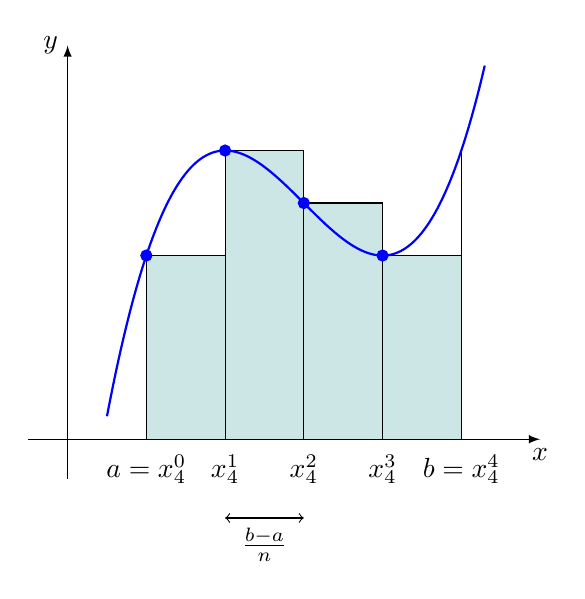
\begin{tikzpicture}[scale=1,declare function={f(\x)=((1/3)*(\x)^(3)-3*(\x)^(2)+8*\x-3;}]
\coordinate (start) at (.8,{f(.8)});
\coordinate (x0) at (1,{f(1)});
\coordinate (x1) at (2,{f(2)});
\coordinate (x2) at (3,{f(3)});
\coordinate (x3) at (4,{f(4)});
\coordinate (x4) at (5,{f(5)});
\coordinate (end) at (5.05,{f(5.05)});
\draw[fill=teal!20!white] (1,0) rectangle (2,{f(1)});
\draw[fill=teal!20!white] (2,0) rectangle (3,{f(2)});
\draw[fill=teal!20!white] (3,0) rectangle (4,{f(3)});
\draw[fill=teal!20!white] (4,0) rectangle (5,{f(4)});
\draw (5,0)--(5,{f(5)});
\draw [-latex] (-0.5,0) -- (6,0) node (xaxis) [below] {$x$};
\draw [-latex] (0,-0.5) -- (0,5) node [left] {$y$};
\foreach \x/\xtext in {1/a=x^0_{4} ,2/x^1_{4}, 3/x^2_{4} , 4/x^3_{4} , 5/b=x^4_{4}}
 \draw[xshift=\x cm] (0pt,3pt) -- (0pt,0pt) 
node[below=2pt,fill=white,font=\normalsize]
  {$\xtext$};
\draw[domain=.5:5.3,samples=200,variable=\x,blue,thick] plot ({\x},{f(\x)});                 
\foreach \n in {0,1,2,3}
\draw[blue,fill=blue] (x\n) circle (2pt) node[font=\normalsize] {$ $};    
\draw[<->] (2,-1)--(3,-1) node[below,midway] {$\frac{b-a}{n}$};      
\end{tikzpicture}
\end{marginfigure}

\begin{preuve}
    
\end{preuve}

\begin{exercice}
    \marginnote[0cm]{\cite{maths-france} Planche no 37. Intégration sur un segment}
    Limites quand $n$ tend vers $+ \infty$ de 
    \begin{multicols}{2}
        \begin{enumerate}
            \item $$\frac{1}{n^3} \sum_{k=1}^n k^2 \sin \frac{k \pi}{n}$$
            \item Soit $a > 0$, 
            $$\left( \frac{1}{n!} \prod_{k=1}^n (a+k) \right)^{1/n}$$
            \item $$\sum_{k=1}^n \frac{n+k}{n^2+k}$$
            \item $$\sum_{k=0}^{n-1} \frac{1}{\sqrt{n^2-k^2}}$$
            \item $$\frac{1}{n \sqrt{n}} \sum_{k=1}^n \left \lfloor \sqrt{k} \right \rfloor$$
            \item $$\sum_{k=1}^n \frac{k^2}{8k^3 + n^3}$$
            \item $$\sum_{k=n}^{2n-1} \frac{1}{2k+1}$$
            \item $$n \sum_{k=1}^n \frac{\me^{-n/k}}{k^2}$$
        \end{enumerate}
    \end{multicols}
\end{exercice}

\begin{solution}
    \begin{enumerate}
        \item 
    \end{enumerate}
\end{solution}

\begin{methode}
    \begin{itemize}
        \item 
    \end{itemize}
\end{methode}

Les sommes de \textsc{Riemann} permettent de calculer des intégrales mais leur convergence est lente comme le montrer l'exercice suivant.

\begin{exercice}
    \marginnote[0cm]{\cite{maths-france} Planche no 37. Intégration sur un segment}
    Soit $f$ une fonction de classe $\mathscr{C}^2$ sur $[0, 1]$. Déterminer le réel $a$ tel que:
    $$\int_0^1 f(t) \d t - \frac{1}{n} \sum_{k=1}^{n-1} f \left( \frac{k}{n} \right) =\limits_{n \to + \infty} \frac{a}{n} + o \left( \frac{1}{n} \right).$$
\end{exercice}

\section{Intégration des relations de comparaisons}
\begin{prop}{}
    Soit $f: \Rp \rightarrow \C$ une fonction continue par morceaux et $g, h:\Rp \rightarrow \Rp$ deux fonctions continues par morceaux, strictement positives. On suppose que $f = o_{+\infty}(g)$ et $f \sim_{+\infty} h$.\\
    \begin{itemize}
        \item Si $g$ et $h$ ne sont pas intégrables sur $\Rp$,
        $$\int_{0}^{x} f = o_{+\infty} \left(\int_{0}^{x} g \right) \text{ et } \int_{0}^{x} f \sim_{+\infty} \int_{0}^{x} h.$$
        \item Si $g$ et $h$ sont intégrables sur $\Rp$,
        $$\int_{x}^{+\infty} f = o_{+\infty} \left(\int_{x}^{+\infty} g \right) \text{ et } \int_{x}^{+\infty} f \sim_{+\infty} \int_{x}^{+\infty} h.$$
    \end{itemize}
\end{prop} 

La démonstration est analogue à celle de la \nameref{sommation_relations_comparaison}

% \section{Transformée de \textsc{Fourier} de la loi normale}
% \input{chapitres/integration/transformee_de_fourier_de_la_loi_normale}

% \section{Intégrale à paramètre dans les bornes}
% \begin{itemize}
    \item On pose $f:x \mapsto \int_{x}^{x^2} \frac{\d t}{\ln (t)}$.
    $$\displaystyle f(x) = \int_{x}^{x^2} \frac{t}{t \ln (t)} \d t \leqslant x^2 \int_{x}^{x^2} \frac{\d t}{t \ln(t)} = x^2 \bigl[ \ln (\ln (t)) \bigr]_x^{x^2} = x^2 \ln(2).$$
\end{itemize}

\section{Intégrale de \textsc{Dirichlet}}
\textcolor{red}{A revoir}
\begin{prop}{}
    L'intégrale de \textsc{Dirichlet} (1829) est l'intégrale de la fonction sinus cardinal sur la demi-droite des réels positifs
    $$\int_{0}^{+\infty} \frac{\sin x}{x} \d x = \frac{\pi}{2}.$$
\end{prop}

\begin{marginfigure}[0cm]
    \begin{tikzpicture}
    
\begin{axis}[
    % width=7.5cm,
    % grid=both,
    xmin=-11,
    xmax=11,
    ymin=-0.25,
    ymax=1.15,
    % ylabel=$\mathrm{sinc}(x)$,
    axis lines=middle,
    axis line style=thick,
    axis line style={-latex},
    xticklabels={},
    xtick={-3*3.141592, -2*3.141592, -3.141592, 3.141592, 2*3.141592, 3*3.141592},
    ytick={0, 1},
    xlabel=$x$,
    every axis x label/.style={at={(current axis.right of origin)},anchor=south},
]
              
  \addplot[domain=-15:15, blue, samples=200, name path=B] plot[thick] {sin(deg(x))/x};

  \path[name path=xaxis]
      (-15,0) -- (\pgfkeysvalueof{/pgfplots/xmax},0);
    \addplot[blue!25, opacity=0.9] fill between[of=xaxis and B];
  
  \node[blue,above left] at (-2,0.5) {$\displaystyle x \mapsto \frac{\sin(x)}{x}$};
\end{axis}
\begin{axis}[
    % width=7.5cm,
    % grid=both,
    xmin=-11,
    xmax=11,
    ymin=-0.25,
    ymax=1.15,
    % ylabel=$\mathrm{sinc}(x)$,
    axis lines=middle,
    % axis line style=thick,
    % axis line style={-latex},
    axis line style={draw=none},
    xticklabels={\contour{white}{$-3\pi$}, \contour{white}{$-2\pi$}, \contour{white}{$-\pi$}, \contour{white}{$\pi$}, \contour{white}{$2\pi$}, \contour{white}{$3\pi$}},
    xtick={-3*3.141592, -2*3.141592, -3.141592, 3.141592, 2*3.141592, 3*3.141592},
    ytick={0, 1},
]
\end{axis}
\end{tikzpicture}
\end{marginfigure}

\begin{preuve}
    \begin{enumerate}
        \item Montrer que $\int_{0}^{1} \frac{\sin (t)}{t} \d t$ est convergente. 
        \item Deux méthodes.
        \begin{itemize}
            \item Montrer que la série de terme général $\int_{n \pi}^{(n+1) \pi} \frac{\sin(t)}{t} \d t$ est convergente. En déduire que $\int_{1}^{+ \infty} \frac{\sin(t)}{t} \d t$ converge. 
            \begin{enumerate}
                \item Montrer que $u_n = \int_{n \pi}^{(n+1) \pi} \frac{\sin(t)}{t} \d t$ est le terme général d'une série alternée. Donc $\sum u_n$ converge.\\
                Attention: on ne peut pas en déduire directement que $\sum\limits_{n=0}^{+ \infty} \int_{n \pi}^{(n+1) \pi} \frac{\sin(t)}{t} \d t = \int_{1}^{+ \infty} \frac{\sin(t)}{t} \d t$ car on n'a pas encore démontrer la convergence du deuxième membre (c.f. relation de \textsc{Chasles}).\\
                \item Il faut montrer la convergence de $\int_{\pi}^{x} \frac{\sin (t)}{t} \d t$. \textcolor{green}{A compléter.}
            \end{enumerate}
            \item On peut aussi procéder par intégration par parties en posant
            $$
            \begin{drcases}                
                u(t) = \frac{1}{t}\\
                v(t) = - \cos(t)
            \end{drcases}
            \mathscr{C}^1 \text{ sur } [1, +\infty].
            $$
            Bien présicer que $u(t)v(t)=-\frac{\cos(t)}{t}$ admet une limite finie en 1 et en $+ \infty$.\\
            \begin{remarque}
                L'intégration par parties préserve la régularité de l'intégrale mais ne préserve pas l'intégrabilité.
            \end{remarque}
        \end{itemize}
        \item On en déduit immédiatement que $\int_{0}^{+ \infty} \frac{\sin (t)}{t} \d t$ converge.
        \item De plus, on peut montrer que cette intégrale est semi-convergente (i.e. elle n'est pas intégrable sur $\Rp$). Pour cela, montrer que pour tout entier naturel $n$, $\int_{n \pi}^{(n+1) \pi} \frac{\sin(t)}{t} \d t \geqslant \frac{2}{(n+1) \pi}$. 
    \end{enumerate}
\end{preuve}

\subsection{Intégrabilité du sinus cardinal sur  \texorpdfstring{$\Rpe$}{R+*}}

\begin{prop}{}
    La fonction sinus cardinal $\mathrm{sinc}:t \mapsto \frac{\sin(t)}{t}$ n'est pas intégrable sur $]0, +\infty[$.
\end{prop}

\begin{preuve}
    \marginnote[0cm]{Source : \href{https://www.agreg-maths.fr/uploads/versions/1175/dirichlet.pdf}{Intégrale de \textsc{Dirichlet} -- Florian \textsc{Dussap}}}
    Soit $N \in \Ne$, alors:
    \begin{align*}
        \int_0^{N \pi} \frac{|\sin x|}{x} \d x &= \sum_{k=0}^{N-1} \int_{k \pi}^{(k+1) \pi} \frac{|\sin x|}{x} \d x \\
        \text{par un changement de variable } &= \sum_{k=0}^{N-1} \int_0^\pi \frac{|\sin x|}{x + k \pi} \d x \\
        &\geqslant \sum_{k=0}^{N-1} \frac{1}{(k+1) \pi} \int_0^\pi \sin x \d x \\
        &\geqslant \frac{2}{\pi} \sum_{k=1}^N \frac{1}{k} \xrightarrow[N \to + \infty]{} + \infty.
    \end{align*}
\end{preuve}

\subsection{Intégrale de \textsc{Dirichlet} via une intégrale à paramètre}

Soit la transformée de \textsc{Laplace} de la fonction sinus cardinal:
$$F:x \to \int_{0}^{+ \infty} \exp(-xt) \frac{\sin (t)}{t} \d t$$
    
\begin{enumerate}
    \item \emph{Montrer que $F$ est définie sur $\Rp$.}
    \begin{itemize}
        \item Si $x > 0$, majorer l'intégrande par $t \mapsto \exp(-xt)$.
        \item Si $x = 0$, montrer le prolongement par continuité de la fonction sinus cardinal en $0$ puis intégrer la fonction sinus cardinal par parties sur $[1, +\infty]$.
    \end{itemize}
    \item \emph{Calculer $F$ sur $\Rpe$, en déduire la valeur de la fonction de \textsc{Dirichlet}}
\end{enumerate}

\subsection{Régularité du sinus cardinal sur $\R$}

\begin{exercice}
    Pour $x$ réel, on pose 
    $$f(x) \defeq
    \begin{cases} 
        \frac{\sin x}{x} &\text{si } x \not= 0 \\ 
        1 &\text{si } x = 0 
    \end{cases}.$$ 
    Montrer que $f$ est de classe $\mathscr{C}^\infty$ sur $\R$.
\end{exercice}

\begin{solution}
    \marginnote[0cm]{fic00126}
    Pour $x$ réel non nul, $f(x) = \sum\limits_{n=0}^{+ \infty} (-1)^n \frac{x^{2n}}{(2n+1)!}$ ce qui reste vrai pour $x = 0$. La fonction $f$ est donc développable en série entière sur $\R$ et en particulier, la fonction $f$ est de classe $\mathscr{C}^\infty$ sur $\R$.
\end{solution}



\section{Intégrales eulériennes}
\marginnote[0mm]{Texte de Pierre-Jean \textsc{Hormière}}
De premières tentatives pour définir $n!$ pour des valeurs non entières remontent à \textsc{Stirling} et Daniel \textsc{Bernoulli}. Dans une lettre à Christian \textsc{Goldbach} du 13 octobre 1729, \textsc{Euler} découvre (ou invente ?) une fonction de variable réelle prolongeant de manière naturelle la fonction $n!$. D'abord introduite comme limite de produits, cette fonction fut plus tard présentée sous forme intégrale et reliée à des fonctions voisines. \\
Les fonctions eulériennes sont les plus importantes \say{ fonctions spéciales } de l'analyse classique, réelle et complexe. \textsc{Legendre} les a nommées, classifiées et étudiées. Elles ont aussi été étudiées par \textsc{Gauss}, \textsc{Binet}, \textsc{Plana}, \textsc{Malmsten}, \textsc{Raabe}, \textsc{Weierstrass}, \textsc{Hankel}, H. \textsc{Bohr}, \textsc{Mollerup}, \textsc{Artin} \dots \\
Il y a bien des façons de prolonger la fonction $n!$ au domaine réel, même en se limitant aux fonctions continues. Une idée naturelle est de partir de la formule $\displaystyle n! = \int_{0}^{+ \infty} t^n \me^{-t} \d t$. Cette forme intégrale de la factorielle suggère de considérer la fonction $\displaystyle F(x)=\int_{0}^{+ \infty} t^x \me^{-t} \d t$. Cette fonction, définie sur $]-1, +\infty[$, prolonge intelligemment la factorielle, en ce sens qu'elle possède des propriétés nombreuses et cohérentes. Par commodité, on considère plutôt $\displaystyle \Gamma(x) = \int_{0}^{+ \infty} t^{x-1} \me^{-t} \d t$.

\subsection{Fonction Gamma d'\textsc{Euler}}

%\begin{marginfigure}[3cm]
%    \begin{tikzpicture}[]

\begin{axis}[
xmin = -4.9, xmax = 5.1, 
%ymin = -3.5, ymax = 3.5,  
restrict y to domain=-6:6,
axis lines = middle,
axis line style={-latex},  
xlabel={$x$}, 
ylabel={$\Gamma(x)$},
%enlarge x limits={upper={val=0.2}},
enlarge y limits=0.05,
x label style={at={(ticklabel* cs:1.00)}, inner sep=5pt, anchor=north},
y label style={at={(ticklabel* cs:1.00)}, inner sep=2pt, anchor=south east},
]

\addplot[color=red, samples=222, smooth, 
domain = 0:5] gnuplot{gamma(x)};

\foreach[evaluate={\N=\n-1}] \n in {0,...,-5}{%
\addplot[color=red, samples=555, smooth,  
domain = \n:\N] gnuplot{gamma(x)};
%
\addplot [domain=-6:6, samples=2, densely dashed, thin] (\N, x);
}%
\end{axis}
\end{tikzpicture}
%    \caption*{\centering Graphe de la fonction Gamma}
%\end{marginfigure}

\begin{defi}
    Pour tout $x$ > 0 réel, la \emph{fonction Gamma d'\textsc{Euler}} est définie par: 
    $$\Gamma(x) \defeq \int_{0}^{+\infty} t^{x-1} \me^{-t} \d t.$$
\end{defi}

\begin{remarque}
    À un changement de variable près, la fonction $\Gamma$ est la \nameref{transformee_laplace} de la fonction $t \mapsto t^x$. 
\end{remarque} 

\begin{prop}
    \begin{itemize}
        \item $\Gamma$ est définie si et seulement si $x>0$.
        \item Pour tout $x > 0$, $\Gamma(x+1) = x\Gamma(x)$. \\
        En particulier, $\forall n \in \N$, $\Gamma(n+1) = n!$. 
    \end{itemize}
\end{prop}

\begin{preuve}
    \begin{itemize}
        \item La fonction $f_x:t \mapsto t^{x-1} \me^{-t}$ est continue sur $]0, + \infty[$ comme produit de fonctions qui y sont continues. La fonction $f_x$ est donc intégrable sur tout segment de $]0, +\infty[$. Il reste à étudier son intégrabilité en $0$ et en $+ \infty$:
        \begin{itemize}
            \item[$\triangleright$] En $+\infty:$ par croissances comparées, $f_x(t) = o_{+\infty} \left(\frac{1}{t^2} \right)$. D'après le théorème de comparaison des fonctions à termes positifs, $f_x$ est intégrable au voisinage de $+\infty$.
            \item[$\triangleright$] En $0$: $f_x(t) \sim_0 t^{x-1}$ qui est intégrable d'après \textsc{Riemann} si et seulement si $1-x < 1$ i.e. si et seulement si $x > 0$.
        \end{itemize}

        \item Soit $x > 0$. Calculons $\Gamma(x+1)$ en effectuant une intégration par parties. Posons $u:t \mapsto \me^{-t}$ et $v:t \mapsto t^x$, toutes deux de classe $\mathscr{C}^1$ sur $\Rp$. Vérifions la convergence du \emph{crochet}:
        \begin{align*}
            \text{par croissances comparées } & \lim_{t \to +\infty} u(t) v(t) = 0, \\
            \text{ comme } x > 0 & \lim_{t \to 0} u(t) v(t) = 0.
        \end{align*}
        Ainsi, d'après le théorème d'intégration par parties généralisées, 
        $$\int_{0}^{+\infty} t^{x-1} \me^{-t} \d t = \underbrace{0}_{\text{crochet}} - \int_{0}^{+\infty} xt^{x-1} (-\me^{-t}) \d t.$$
        soit 
        $$\Gamma(x+1) = x \Gamma(x).$$
        En particulier, $\Gamma(1) = 1$ et pour tout $n \in \Ne, \Gamma(n+1) = n \Gamma(n)$. Donc
        $$\forall n \in \Ne, \Gamma(n+1) = n!$$
        Cette fonction, introduite en 1729 par le mathématicien suisse, prolonge la fonction factorielle à l'ensemble des réels strictement positifs.
    \end{itemize}
\end{preuve}

\marginnote[-5cm]{
    \begin{kaobox}[frametitle=Théorème (Intégration par parties généralisées)]
        \cite{acamanes}\\
        Soient $f$ et $g$ deux fonctions de classe $\mathscr{C}^1$ sur $I$. Si la fonction $fg$ a une limite finie en $a$ et en $b$, alors les intégrales
        $$\int_a^b f'(t)g(t) \d t \text{ et } \int_a^b f(t) g'(t) \d t$$
        sont de même nature. Si ces quantités sont convergentes, en notant
        \begin{align*}
            [f(t)g(t)]_a^b = \lim_{x \to b^-} (f(x)g(x)) - \lim_{x \to a^+}(f(x)g(x)),
        \end{align*}
        on obtient la relation
        $$\int_a^b f'(t) g(t) \d t = [f(t)g(t)]_a^b - \int_a^b f(t) g'(t) \d t.$$
    \end{kaobox}
}

\underline{Dérivées successives:} \\
Utiliser une domination locale sur un segment $[a, A] \subset \R_+^\star$ par la fonction:
$$\varphi_k:t \mapsto 
\begin{cases}
    |\ln t |^k \me^{-t} t^{a-1}, & \text{si } t \in ]0, 1] \\
    |\ln t |^k \me^{-t} t^{A-1}, & \text{si } t > 1
\end{cases}
$$
$$\boxed{\forall k \in \N,\ \forall x \in \R_+^\star,\ \Gamma^{(k)}(x) = \int_{0}^{+\infty} (\ln t)^k t^{x-1} \me^{-t} \d t}$$

\underline{Exercice:} \url{https://share.miple.co/content/t8BIcXSjdEslq}

\subsection{Fonction bêta}
\begin{defi}
    Pour tout $(p,q) \in \N^2$, on note
    $$I_{p,q} \defeq \int_{0}^{1} t^p (1-t)^q \d t$$
\end{defi}

\begin{prop}
    Pour tout $(p,q) \in \N^2$,
    $$I_{p,q} = \frac{p! q!}{(p + q + 1)!}.$$
\end{prop}

\begin{preuve}
    Soit $(p,q) \in \N^2$. Nous allons déterminer une relation entre $I_{p,q}$ et $I_{p+1, q-1}$ grâce en faisant une intégration par parties. \\
    On pose $u:t\mapsto \frac{1}{p+1} t^{p+1}$ et $v:t\mapsto (1-t)^q$, toutes deux de classe $\mathscr{C}^1$ sur $[0, 1]$. Alors, 
    \begin{align*}
        I_{p,q} &= \left[ \frac{1}{p+1}t^{p+1} \times (1-t)^q \right]_0^1 + \frac{q}{p+1} \int_0^1 t^{p+1} (1-t)^{q-1} \d t \\
        I_{p,q} &= \frac{q}{p+1} I_{p+1, q-1}.
    \end{align*}
    On en déduit que 
    \begin{align*}
        I_{p,q} &= \frac{q}{p+1} \times \frac{q-1}{p+2} \times \cdots \times \frac{1}{p+q} I_{p+q,0} \\
        I_{p,q} &= \frac{p! q!}{(p + q + 1)!}.
    \end{align*}
\end{preuve}

\url{https://fr.wikipedia.org/wiki/Intégrale_d'Euler} \\
\cite{calcul_infinitesimal} Chapitre IV, 3 Intégrales eulériennes, page 125.

\begin{exercice}
    \cite{acamanes} \\
    Déterminer la nature de la série $\sum I_{n,n}$ et, le cas échéant, calculer sa somme. 
\end{exercice}

\begin{solution}
\end{solution}


\section{Intégrale de \textsc{Gauss}}
\begin{tcolorbox}
    $$\int_{0}^{+\infty} \me^{-x^2}\ \d x = \frac{\sqrt{\pi}}{2}$$
\end{tcolorbox}

\section{Intégrale de \textsc{Wallis}} \label{integrale_wallis}
\todoinline{Pour moi il faut faire le lien quelque part avec la formule de Stirling.}

\begin{defi}{Intégrale de \textsc{Wallis}}
    $$\Wallis_n \defeq \int_{0}^{\frac{\pi}{2}} \sin(x)^n \d x = \int_{0}^{\frac{\pi}{2}} \cos(x)^n \d x$$
\end{defi}

\begin{prop}{} \labprop{prop_wallis}
    $$\Wallis_{2p} = \frac{\binom{2p}{p}}{2^{2p}}\frac{\pi}{2} \text{ et } \Wallis_{2p+1} = \frac{2^{2p} (p!)^2}{(2p+1)!}$$
    $$\Wallis_{n+1} \sim \Wallis_n \qquad \Wallis_n \sim \sqrt{\frac{\pi}{2n}}$$
    $$\Wallis_n \Wallis_{n+1} = \frac{\pi}{2(n+1)}$$
\end{prop}

\begin{preuve}
    Calculons $\Wallis_{n+2}$ en effectuant une intégration par parties. On pose $u(t) \defeq - \cos(t)$ et $v(t) \defeq \sin(t)^{n+1}$, toutes deux de classe $\mathscr{C}^1$ sur $\left[0, \frac{\pi}{2} \right]$. 
    \begin{align*}
        \Wallis_{n+2} &= \underbrace{\left[ -\cos(t) \sin(t)^{n+1} \right]_0^{\pi/2}}_{=0} + (n+1) \int_0^{\pi/2} \cos(t)^2 \sin(t)^n \d t \\
        &= (n+1) \int_0^{\pi/2} \big(1 - \sin(t)^2 \big) \sin(t)^n \d t \\
        &= (n+1) \Wallis_n - (n+1) \Wallis_{n+2} \\
        \text{soit } (n+2) \Wallis_{n+2} &= (n+1) \Wallis_n.
\end{align*}
Soit $p \in \N$. D'après la relation précédente, 
\begin{figure*}[h!]
\begin{multicols}{2}
\begin{align*}
    \Wallis_{2p} &= \frac{2p-1}{2p} \Wallis_{2p-2} \\
    &= \frac{2p-1}{2p} \times \frac{2p-3}{2p-2} \times \cdots \times \frac{1}{2} \times \underbrace{\Wallis_0}_{=\pi/2} \\
    &= \frac{\prod\limits_{k=1}^p (2k+1)}{\prod\limits_{k=1}^{p+1} (2k)} \frac{\pi}{2} \\
    &= \frac{\left[\prod\limits_{k=1}^p (2k+1) \right] \times \left[ \prod\limits_{k=1}^{p+1} (2k) \right]}{\left[\prod\limits_{k=1}^{p+1} (2k) \right]^2} \frac{\pi}{2} \\
    \Wallis_{2p} &= \frac{(2p)!}{2^{2p}(p!)^2} \frac{\pi}{2}.
\end{align*}
\begin{align*}
    \Wallis_{2p+1} &= \frac{2p}{2p+1} \Wallis_{2p-1} \\
    &= \frac{2p}{2p+1} \times \frac{2p-2}{2p-1} \times \cdots \times \frac{2}{3} \times \underbrace{\Wallis_1}_{=1} \\
    &= \frac{\prod\limits_{k=1}^p (2k)}{\prod\limits_{k=0}^p (2k+1)} \\
    &= \frac{\left[ \prod\limits_{k=1}^p (2k) \right]^2}{\left[ \prod\limits_{k=0}^p (2k+1) \right] \left[ \prod\limits_{k=1}^p (2k) \right]} \\
    \Wallis_{2p+1} &= \frac{2^{2p}(p!)^2}{(2p+1)!}.
\end{align*}
\end{multicols}
\end{figure*}
\end{preuve}

\subsection{Séries génératrices}

\todoinline{C'est rigolo ! Est-ce qu'on pourrait retrouver l'expression de $W_n$ à l'aide d'un produit de DSE ? Il y a aussi une application ici : https://math-os.com/coefficient-binomial-central/}

\textcolor{red}{Ajouter un texte d'introduction}

\begin{prop}{}
    \marginnote[0cm]{Source : \href{https://fr.wikipedia.org/wiki/Intégrale_de_Wallis}{Intégrale de \textsc{Wallis} -- \textsf{wikipedia.org}}}
    La série génératrice des termes pairs est 
    $$\sum_{p=0}^\infty \Wallis_{2p} x^{2p} = \frac{\pi}{2} \frac{1}{\sqrt{1-x^2}}.$$
    La série génératrice des termes impairs est 
    $$\sum_{p=0}^\infty \Wallis_{2p+1} x^{2p+1} = \frac{\arcsin x}{\sqrt{1-x^2}}.$$
\end{prop}

\begin{exercice}
    Soit $x \in ]0,1[$. Calculer $\sum\limits_{n=0}^\infty (-1)^n \Wallis_n$ puis $\sum\limits_{n=0}^\infty \Wallis_n x^n$.
\end{exercice}

\begin{solution}
    \marginnote[0cm]{Source : \href{http://exo7.emath.fr/ficpdf/fic00126.pdf}{Exercices de Jean-Louis \textsc{Rouget} (fic00126) -- \textsf{http://exo7.emath.fr}}}
    D'après \vrefprop{prop_wallis}, $\Wallis_n \sim \sqrt{\frac{\pi}{2n}}$ et la règle de \textsc{d'Alembert} fournit $R = 1$. Soit $x \in ]-1, 1[$. \\
    Pour tout $t \in \left[ 0, \frac{\pi}{2} \right]$ et tout entier naturel $n$, $|x^n \cos^n t| \leqslant |x|^n$. Comme la série numérique de terme général $|x|^n$ converge, la série de fonctions de terme général $t \mapsto x^n \cos^n t$ est normalement convergente et donc uniformément convergente sur le segment $\left[ 0, \frac{\pi}{2} \right]$. D'après le théorème d'intégration terme à terme sur un segment, 
    \begin{align*}
        \sum_{n=0}^{+ \infty} \Wallis_n x^n &= \sum_{n=0}^{+ \infty} \left[ x^n \int_0^{\pi/2} \cos^n t \d t \right] = \int_0^{\pi/2} \left( \sum_{n=0}^{+\infty} x^n \cos^n t \right) \d t \\
        &=\int_0^{\pi/2} \frac{1}{1 - x \cos t} \d t \\
        &= \int_0^1 \frac{1}{1 - x \frac{1-u^2}{1+u^2}} \frac{2}{1 + u^2} \d u \quad \text{en posant } u = \tan \frac{t}{2} \\
        &= 2 \int_0^1 \frac{1}{(1+x)u^2 + (1-x)} \d u \\
        &= 2 \times \frac{1}{1+x} \times \frac{1}{\sqrt{\frac{1-x}{1+x}}} \left[ \arctan \left( \frac{u}{\sqrt{\frac{1-x}{1+x}}} \right) \right]_0^1 \\
        \sum_{n=0}^{+ \infty} \Wallis_n x^n &= \frac{2}{\sqrt{1-x^2}} \arctan \sqrt{\frac{x+1}{x-1}}.
    \end{align*}
\end{solution}

\subsection{Calcul de l'intégrale de \textsc{Gauss}}
\marginnote[0cm]{Source : \href{https://fr.wikipedia.org/wiki/Intégrale_de_Wallis}{Intégrale de \textsc{Wallis} -- \textsf{wikipedia.org}}}
On peut aisément utiliser les intégrales de \textsc{Wallis} pour calculer l'intégrale de \text{Gauss}. \\
On utilise pour cela l'encadrement suivant, issu de la construction de la fonction exponentielle par la méthode d'\textsc{Euler}: pour tout entier $n > 0$ et tout réel $u \in ]-n, n[$, 
$$\left(1 + \frac{u}{n} \right)^n \leqslant \e^u \leqslant \left( 1 - \frac{u}{n} \right)^{-n}.$$
Posant alors $u = -x^2$, on obtient:
$$\int_0^{\sqrt{n}} \left( 1 - \frac{x^2}{n} \right)^n \d x \leqslant \int_0^{\sqrt{n}} \e^{-x^2} \d x \leqslant \int_0^{\sqrt{n}} \left( 1 + \frac{x^2}{n} \right)^{-n} \d x.$$
Or les intégrales d'encadrement sont liées aux intégrales de \textsc{Wallis}. Pour celle de gauche, il suffit de poser $x = \sqrt{n} \sin t$ ($t$ variant de $0$ à $\pi/2$). Quant à celle de droite, on peut poser $x = \sqrt{n} \tan t$ ($t$ variant de $0$ à $\pi/4$) puis majorer par l'intégrale de $0$ à $\pi/2$. On obtient ainsi:
$$\sqrt{n} \Wallis_{2n+1} \leqslant \int_0^{\sqrt{n}} \e^{-x^2} \d x \leqslant \sqrt{n} \Wallis_{2n-2}.$$
Par le théorème des gendarmes, on déduit alors de l'équivalent de $\Wallis_n$ que
$$\int_0^{+ \infty} \e^{-x^2} \d x = \frac{\sqrt{\pi}}{2}.$$

\subsection{Volume d'une boule en dimension \texorpdfstring{$n$}{n}}

\begin{exercice}
    \marginnote[0cm]{Source : \cite{fmaalouf}}
    Pour $n \in \Ne$ et $R \in \Rpe$ on désigne par $V_n(R)$ le volume de la boule de $\R^n$ de centre $O$ et de rayon $R$, 
    $$V_n(R) \defeq \idotsint_{x_1^2 + \cdots + x_n^2 \leqslant R^2} \d x_1 \cdots \d x_n.$$
    Montrer que pour tout $p \in \Ne$, 
    $$V_{2p}(R) = \frac{\pi^p R^{2p}}{p!}.$$
\end{exercice}

\todoinline{Ajouter une preuve.}

\todoarmand{Les exercices 4 et 5 de \url{http://exo7.emath.fr/ficpdf/fic00143.pdf} donnent les liens entre calcul de la surface de la sphère unité de $\R^n$, son volume, la fonction Gamma et les intégrales de Wallis.}

\subsection{\textsc{Grain de raisin}: Produit de \textsc{Wallis}}

\begin{prop}{Produit de \textsc{Wallis}}
    $$\prod_{n=1}^{\infty} \frac{4n^2}{4n^2-1} = \frac{\pi}{2}$$
\end{prop}

\begin{preuve}
    Puisque $\Wallis_{2n} \sim \Wallis_{2n+1}$, 
    $$\lim_{n \to +\infty} \frac{\Wallis_{2n+1}}{\Wallis_{2n} / \frac{\pi}{2}} = \frac{\pi}{2}.$$
    Or d'après le calcul des intégrales de \textsc{Wallis}:
    $$\frac{\Wallis_{2n+1}}{\Wallis_{2n} / \frac{\pi}{2}} = \frac{\frac{2^{2p}(p!)^2}{(2p+1)!}}{\frac{(2p)!}{2^{2p}(p!)^2}} = \prod_{k=1}^n \frac{4k^2}{4k^2-1}.$$
\end{preuve}

\section{Théorème de \textsc{Fubini}}

\marginnote[-2mm]{Ce théorème a été démontré par le mathématicien italien Guido \textsc{Fubini} en 1907.}
\begin{theo}{\textsc{Fubini}}
    Soit $f: [a,b] \times [c, d] \to \K$ une application continue. Alors,
    $$\int_{a}^{b} \left ( \int_{c}^{d} f(x,y) \d y \right) \d x = \int_{c}^{d} \left ( \int_{a}^{b} f(x,y) \d x \right) \d y.$$
\end{theo}

\begin{marginfigure}[5cm]
    \centering
    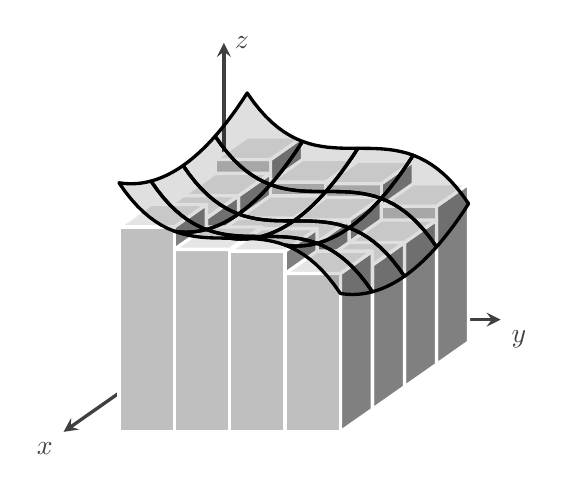
\begin{tikzpicture}[
  x=(215:2em/sqrt 2), y=(0:2em), z=(90:2em),
  declare function={f(\x,\y)=((\x-3)^2+(-\y+3)^3)/8+3;}, 
  very thick, line join=round]
\draw [-stealth, black!75] (0,0,0) -- (5,0,0) node [below left] {$x$};
\draw [-stealth, black!75] (0,0,0) -- (0,5,0) node [below right] {$y$};
\draw [-stealth, black!75] (0,0,0) -- (0,0,5) node [right] {$z$};
\foreach \x in {1,...,4}
  \foreach \y [evaluate={\j=\x+.5; \i=\y+.5; \k=f(\j,\i);}] in {1,...,4}{
    \path [fill=black!50, draw=white] (\x, \y+1, 0) -- (\x+1, \y+1, 0) -- 
      (\x+1, \y+1, \k) -- (\x, \y+1, \k) -- cycle;
    \path [fill=black!25, draw=white] (\x+1, \y, 0) -- (\x+1, \y+1, 0) -- 
      (\x+1, \y+1, \k) -- (\x+1, \y, \k) -- cycle;
    \path [fill=black!10, draw=white] (\x, \y, \k)  -- (\x+1, \y, \k) -- 
      (\x+1, \y+1, \k) -- (\x, \y+1, \k) -- cycle;
  }
 \foreach \x in {1,...,4}
   \foreach \y in {1,...,4}{
 \draw [black, fill=black, fill opacity=0.125, 
    domain=0:1, samples=10, variable=\t] 
    plot (\x+\t, \y, {f(\x+\t,\y)}) -- 
    plot (\x+1, \y+\t, {f(\x+1,\y+\t)}) -- 
    plot (\x+1-\t, \y+1, {f(\x+1-\t,\y+1)}) --
    plot (\x, \y+1-\t, {f(\x,\y+1-\t)}) -- cycle;
  }
\end{tikzpicture}
    \caption*{\centering Cette figure ne correspond pas au théorème de \textsc{Fubini}}
\end{marginfigure}

Nous allons voir la démonstration de ce résultat sous forme d'exercice.

\begin{exercice}
    Pour tout $(x, t) \in [a, b] \times [c, d]$ on pose 
    $$\varphi(x, t) \defeq \int_{a}^{x} f(u, t) \d u.$$
    \begin{enumerate}
        \item Montrer que pour tout $x \in [a, b]$, l'application $t \mapsto \varphi(x, t)$ est continue sur $[c, d]$.
        \item On pose alors, pour tout $x  \in [a, b]$ 
        $$\psi(x) \defeq \int_{c}^{d} \varphi(x, t) \d t.$$
        Montrer que $\psi$ est de classe $\mathscr{C}^1$ sur $[a, b]$, préciser $\psi'$.
        \item En déduire:
        $$\forall x \in [a, b],\ \int_{a}^{x} \left ( \int_{c}^{d} f(u,t) \d t \right) \d u = \int_{c}^{d} \left ( \int_{a}^{x} f(u,t) \d u \right) \d t.$$
    \end{enumerate}
\end{exercice}

\marginnote[0cm]{Correction du sujet Mines Maths 2 PSI 2021 par Doc Solus.} 
\begin{solution}
    \begin{enumerate}
        \item Application du théorème de continuité des intégrales à paramètre. \\
        Pour la domination : $f$ est continue sur une partie fermée bornée de $\R^2$, donc d'après le théorème des bornes, $f$ est bornée sur $[a, b] \times [c, d]$ par une constante $M \in \Rp$.
        \item Application du théorème de dérivation des intégrales à paramètre à la fonction $x \mapsto \int_{c}^{d} \varphi(x, t) \d t$:
        \begin{itemize}
            \item $\forall t \in [c, d],\ x \mapsto \varphi(x, t)$ est de classe $\mathscr{C}^1$ sur $[a, b]$ car c'est la primitive s'annulant en $a$ de la fonction continue $x \mapsto f(x, t)$. 
            \item $\frac{\partial \varphi}{\partial x}(x, t) = f(x, t)$
            \item La domination se fait par le même constante $M$ que précédemment. 
        \end{itemize}
        $$\forall x \in [a, b] \quad \psi'(x) = \int_{c}^{d} f(x, t) \d t.$$
        \item Soit $x \in [a, b]$. D'une part,
        $$\psi(x) = \int_{c}^{d} \left ( \int_{a}^{x} f(u,t) \d u \right) \d t.$$
        D'autre part, d'après la question précédente et le théorème fondamental de l'analyse, 
        \begin{align*}
            \int_{a}^{x} \left ( \int_{c}^{d} f(u,t) \d t \right) \d u &= \int_{a}^{x} \psi'(u) \d u  = \psi(x) - \psi(a) \\
            \text{Or } \psi(a) &= \int_{c}^{d} \varphi(a, t)\ \d t \\
            \text{et } \forall t \in [c, d] \quad \varphi(a, t) &= \int_{a}^{a} f(u, t) \d u = 0
        \end{align*}
        d'où $\psi(a) = 0$ et le résultat. \\
        En particulier, pour $x = b$ on obtient le résultat final.
    \end{enumerate}
\end{solution}    


\section{Transformée de \textsc{Laplace}} 
\label{transformee_laplace}
La transformation de \textsc{Laplace} généralise la transformation de \textsc{Fourier} qui est également utilisée pour résoudre les équations différentielles : contrairement à cette dernière, elle tient compte des conditions initiales et peut ainsi être utilisée en théorie des vibrations mécaniques ou en électricité dans l'étude des régimes forcés sans négliger le régime transitoire. De manière générale, ses propriétés vis-à-vis de la dérivation permettent un traitement plus simple de certaines équations différentielles, et elle est de ce fait très utilisée en automatique. \\
Dans ce type d'analyse, la transformation de \textsc{Laplace} est souvent interprétée comme un passage du domaine temps, dans lequel les entrées et sorties sont des fonctions du temps, dans le domaine des fréquences, dans lequel les mêmes entrées et sorties sont des fonctions de la \say{ fréquence } (complexe) $p$. Ainsi; il est possible d'analyser simplement l'effet du système sur l'entrée pour donner la sortie en matière d'opérations algébriques simples (cf. théorie des fonctions de transfert en électronique ou en mécanique). 

\begin{defi}{Transformée de \textsc{Laplace}}
    Pour tout fonction $f \in \mathscr{C}(\Rp, \R)$, on note, lorsqu'elle converge, 
    $$\mathscr{L}(f)(p) \defeq \int_{0}^{+ \infty} \e^{-pt} f(t) \d t.$$
    La fonction $\mathscr{L}(f)$ est la \emph{transformée de \textsc{Laplace} de f}.
\end{defi}

\marginnote[0cm]{Sources : \cite{exos_oraux} + \cite{acamanes} (Exercice cerise Ch. 12)}
\underline{Démonstration du théorème de la valeur finale:}
\begin{itemize}
    \item Généralisation classique du théorème des bornes $\leadsto$ $f$ est bornée
    \item Changement de variable: $\varphi: u \mapsto \frac{u}{p}$
    \item Caractérisation séquentielle de la limite
    \item Théorème de convergence dominée
\end{itemize}



\section{Exercice oral}
\begin{exercice}
    On pose
    $$F:x \mapsto \int_x^{+\infty} \frac{\me^{-t}}{t} \d t.$$
    \begin{enumerate}
        \item Déterminer l'ensemble de définition de $F$. Étudier brièvement le comportement de la fonction $F$ et tracer sa courbe représentative.
        \item Déterminer un  équivalent de $F$ en $+\infty$.
        \item Montrer que $F(1) - F(x) - \ln x$ converge vers un réel. (pas sûr de cette question).
    \end{enumerate}
\end{exercice}

%\begin{enumerate}
%    \item $D = ]0, + \infty[$.
%    \item Intégration par parties ou comparaison série / intégrale: $F(x) \sim_{+\infty} \frac{\me^{x}}{x}$. \\
%    \url{https://www.bibmath.net/ressources/index.php?action=affiche&quoi=bde/analyse/integration/integralesimpropres&type=fexo} exercice 38. (à réécrire)\\
%    On remarque d'abord que $\int_{1}^{+\infty} \frac{\me^{-t}}{t} \d t$ converge: en effet, la fonction $t \mapsto \frac{\me^{-t}}{t}$ est continue et positive sur $[1, + \infty[$ et $\lim\limits_{t \to +\infty} t^2 \frac{\me^{-t}}{t} = 0$. On intègre ensuite par parties, en intégrant $t \mapsto \me^{-t}$ et en dérivant $\t \mapsto \frac{1}{t}$. On obtient, pour $x > 1$, 
%    $$\int_x^{+ \infty} \frac{\me^{-t}}{t} \d t = \left[ -\frac{\me^{-t}}{t} \right]_x^{+\infty} - \int_x^{+\infty} \frac{\me^{-t}}{t^2} \d t$$
%    $$\int_x^{+ \infty} \frac{\me^{-t}}{t} \d t= \frac{\me^{-x}}{x} - \int_x^{+\infty} \frac{\me^{-t}}{t^2} \d t.$$
%    Or, au voisinage de $+ \infty$, 
%    $$\frac{\me^{-t}}{t^2} = o\left( \frac{\me^{-t}}{t} \right).$$
%    Par intégration des relations de comparaison (les fonctions sont positives et intégrables), on trouve
%    $$\int_x^{+\infty} \frac{\me^{-t}}{t^2} \d t = o_{+\infty} \left( \int_x^{+\infty} \frac{\me^{-t}}{t} \d t \right).$$
%    On en déduit que
%    $$\int_x^{+\infty} \frac{\me^{-t}}{t} \d t \sim_{+\infty} \frac{\me^{-x}}{x}.$$
%    \item À faire.
%\end{enumerate}

\section{Version intégrale du lemme de \textsc{Cesàro}}
\begin{lemme}
    Soit $f$ une fonction continue telle que $\lim\limits_{+\infty} f = \ell$. Alors 
    $$\lim_{x \to + \infty} \frac{1}{x} \int_0^x f(t) \d t = \ell.$$
\end{lemme}

\begin{preuve}
    La démonstration est directement adaptée de celle de la version discrète. 
    Soit $\varepsilon > 0$. Comme la fonction $f$ converge vers $\ell$ en $+ \infty$, il existe $x_0 \in \Rp$ tel que pour tout $x \geqslant x_0,\ |f(x) - \ell| \leqslant \varepsilon$. \\
    Soit $x > x_0$,
    \begin{align*}
        \left| \frac{1}{x} \int_0^x f(t) \d t - \ell \right| &= \left| \frac{1}{x} \int_0^x (f(t) - \ell) \d t \right| \\
        \text{par l'inégalité triangulaire} &\leqslant \frac{1}{x} \int_0^x |f(t) - \ell| \d t \\
        &\leqslant \frac{1}{x} \Bigg( \underbrace{\int_{0}^{x_0} |f(t) - \ell| \d t}_{\defeq K} + \int_{x_0}^{x} \underbrace{|f(t) - \ell|}_{\leqslant \varepsilon} \d t \Bigg) \\
        &\leqslant \frac{K}{x} + \varepsilon
    \end{align*}
    Or $\lim\limits_{x \to \infty} \frac{K}{x} = 0$ donc il existe $x_1 \in \Rp$ tel que pour tout $x \geqslant x_1, \left| \frac{K}{x} \right| \leqslant \varepsilon$. \\
    Ainsi pour tout $x \geqslant \max \{ x_0, x_1 \}$, 
    $$\left| \frac{1}{x} \int_0^x f(t) \d t - \ell \right| \leqslant 2 \varepsilon.$$
    On en déduit le résultat. 
\end{preuve}

\section{Sinus cardinal}

\begin{exercice}
    Pour $x$ réel, on pose 
    $$f(x) \defeq
    \begin{cases} 
        \frac{\sin x}{x} &\text{si } x \not= 0 \\ 
        1 &\text{si } x = 0 
    \end{cases}.$$ 
    Montrer que $f$ est de classe $\mathscr{C}^\infty$ sur $\R$.
\end{exercice}

\begin{solution}
    \marginnote[0cm]{fic00126}
    Pour $x$ réel non nul, $f(x) = \sum\limits_{n=0}^{+ \infty} (-1)^n \frac{x^{2n}}{(2n+1)!}$ ce qui reste vrai pour $x = 0$. La fonction $f$ est donc développable en série entière sur $\R$ et en particulier, la fonction $f$ est de classe $\mathscr{C}^\infty$ sur $\R$.
\end{solution}